\hypertarget{interface_t_p_parameter_data_scaling}{
\section{TPParameterDataScaling Class Reference}
\label{interface_t_p_parameter_data_scaling}\index{TPParameterDataScaling@{TPParameterDataScaling}}
}
{\tt \#import $<$TPParameterDataScaling.h$>$}

Inheritance diagram for TPParameterDataScaling::\begin{figure}[H]
\begin{center}
\leavevmode
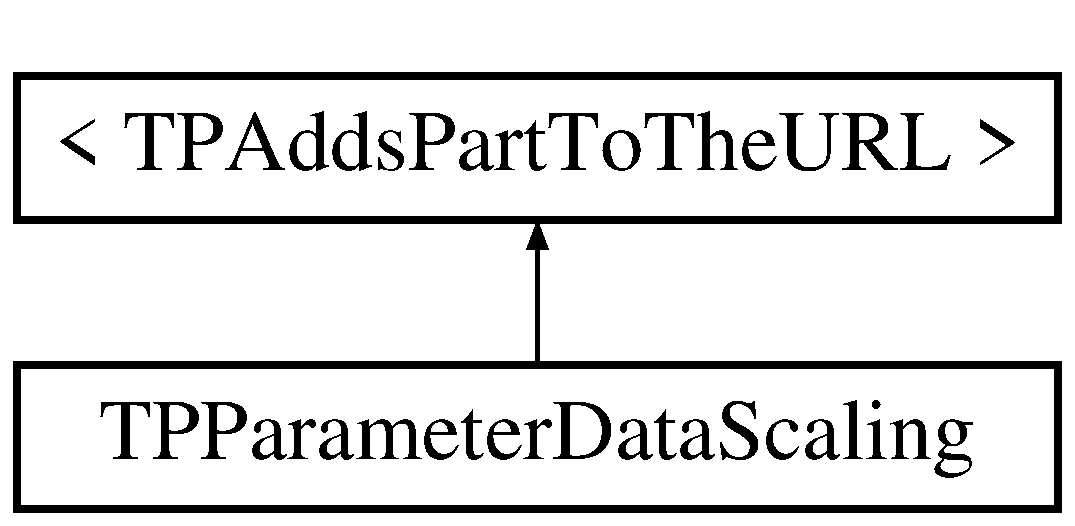
\includegraphics[height=2cm]{interface_t_p_parameter_data_scaling}
\end{center}
\end{figure}
\subsection*{Public Member Functions}
\begin{CompactItemize}
\item 
(void) - \hyperlink{interface_t_p_parameter_data_scaling_3dfe9bc7aed1db751668d2b35ed5f96a}{setValueForDataSet:minValue:maxValue:}
\item 
(NSNumber $\ast$) - \hyperlink{interface_t_p_parameter_data_scaling_5a9973137a688517df307f31c3a0897f}{minValueForDataSet:}
\item 
(NSNumber $\ast$) - \hyperlink{interface_t_p_parameter_data_scaling_ba2b88c8204e29d01147545b935e5af1}{maxValueForDataSet:}
\end{CompactItemize}


\subsection{Detailed Description}
This class is responsible for data scaling 

\subsection{Member Function Documentation}
\hypertarget{interface_t_p_parameter_data_scaling_ba2b88c8204e29d01147545b935e5af1}{
\index{TPParameterDataScaling@{TPParameterDataScaling}!maxValueForDataSet:@{maxValueForDataSet:}}
\index{maxValueForDataSet:@{maxValueForDataSet:}!TPParameterDataScaling@{TPParameterDataScaling}}
\subsubsection[{maxValueForDataSet:}]{\setlength{\rightskip}{0pt plus 5cm}- (NSNumber $\ast$) maxValueForDataSet: (NSInteger) {\em index}}}
\label{interface_t_p_parameter_data_scaling_ba2b88c8204e29d01147545b935e5af1}


Returns the max value for a given index \begin{Desc}
\item[Parameters:]
\begin{description}
\item[{\em index}]index of the max value to return \end{description}
\end{Desc}
\begin{Desc}
\item[Returns:]max value \end{Desc}
\hypertarget{interface_t_p_parameter_data_scaling_5a9973137a688517df307f31c3a0897f}{
\index{TPParameterDataScaling@{TPParameterDataScaling}!minValueForDataSet:@{minValueForDataSet:}}
\index{minValueForDataSet:@{minValueForDataSet:}!TPParameterDataScaling@{TPParameterDataScaling}}
\subsubsection[{minValueForDataSet:}]{\setlength{\rightskip}{0pt plus 5cm}- (NSNumber $\ast$) minValueForDataSet: (NSInteger) {\em index}}}
\label{interface_t_p_parameter_data_scaling_5a9973137a688517df307f31c3a0897f}


Returns the min value for a given index \begin{Desc}
\item[Parameters:]
\begin{description}
\item[{\em index}]index of the min value to return \end{description}
\end{Desc}
\begin{Desc}
\item[Returns:]min value \end{Desc}
\hypertarget{interface_t_p_parameter_data_scaling_3dfe9bc7aed1db751668d2b35ed5f96a}{
\index{TPParameterDataScaling@{TPParameterDataScaling}!setValueForDataSet:minValue:maxValue:@{setValueForDataSet:minValue:maxValue:}}
\index{setValueForDataSet:minValue:maxValue:@{setValueForDataSet:minValue:maxValue:}!TPParameterDataScaling@{TPParameterDataScaling}}
\subsubsection[{setValueForDataSet:minValue:maxValue:}]{\setlength{\rightskip}{0pt plus 5cm}- (void) setValueForDataSet: (NSInteger) {\em index}\/ minValue: (NSNumber $\ast$) {\em min}\/ maxValue: (NSNumber $\ast$) {\em max}}}
\label{interface_t_p_parameter_data_scaling_3dfe9bc7aed1db751668d2b35ed5f96a}


Set a new scaling value for a specified index \begin{Desc}
\item[Parameters:]
\begin{description}
\item[{\em index}]dataset to scale\par
 (e.g. line1 = index 0, line2 = index1,...) \item[{\em min}]min value \item[{\em max}]max value \end{description}
\end{Desc}


The documentation for this class was generated from the following files:\begin{CompactItemize}
\item 
TPParameterDataScaling.h\item 
TPParameterDataScaling.m\end{CompactItemize}
